%\documentclass[../main.tex]{subfiles}
% !TeX root = ../main.tex

\section{Introdução}

\begin{figure}
  \begin{center}
    \includegraphics[width=0.95\textwidth]{figures/}
  \end{center}
  \caption{}\label{fig:}
\end{figure}


\begin{align}
    y &= x^{2} +\int_{1}^{2} \lambda \partial x \\
    x &= a_{0} + \sum_{n=1}^{\infty} a_{n} \cos\left(n\frac{\pi}{2} t\right) +b_{n} \sin(n\omega_0 t) \notag \\
    \frac{Y(s)}{U(s)} &= \frac{K\omega_0^2}{s^2 +2\zeta\omega_0 s +\omega_0^2} \\
    u(t) &= k_p e(t) +k_i\int e(t) dt +k_d \frac{de(t)}{dt} \label{eq:one}
\end{align}


\begin{align}
     y=\begin{cases}
 1, & \text{ se }\quad x= 0,\\
 2, & \text{ se }\quad x= 10,\\
 3, & \text{ se }\quad x= 20.
\end{cases}
\end{align}

\begin{align}
    \dot{x} &= \begin{bmatrix}
0 & 1 \\
-2 & -3 \\
\end{bmatrix} x + \begin{bmatrix}
0 \\
1
\end{bmatrix} u \\
y &= \begin{bmatrix}
0 & 1 \\
\end{bmatrix} x
\end{align}





Na introdução $\nicefrac{Y(s)}{U(s)} = \nicefrac{K\omega_0^2}{s^2}$ a equipe tem que informar o que foi proposto para o projeto de forma clara e dizer, também de forma clara, como as diferentes disciplinas estudadas até aqui se relacionam dentro do projeto escolhido para ser trabalhado. 

\begin{table}[H]
  \centering
  \caption{Characteristics of feeder JSL07}
    \begin{tabular}{cc}
    \toprule
    \textbf{Description} & \textbf{Quantity} \\
    \midrule
    Medium voltage segments & 148 \\
    Low voltage segments & 171 \\
    Distribution transformer units & 24 \\
    Medium voltage transformer units & 13 \\
    Low voltage transformer units & 604 \\
    \bottomrule
    \end{tabular}%
  \label{tab:jsl07}%
\end{table}%

\begin{figure}[H]
    \centering
    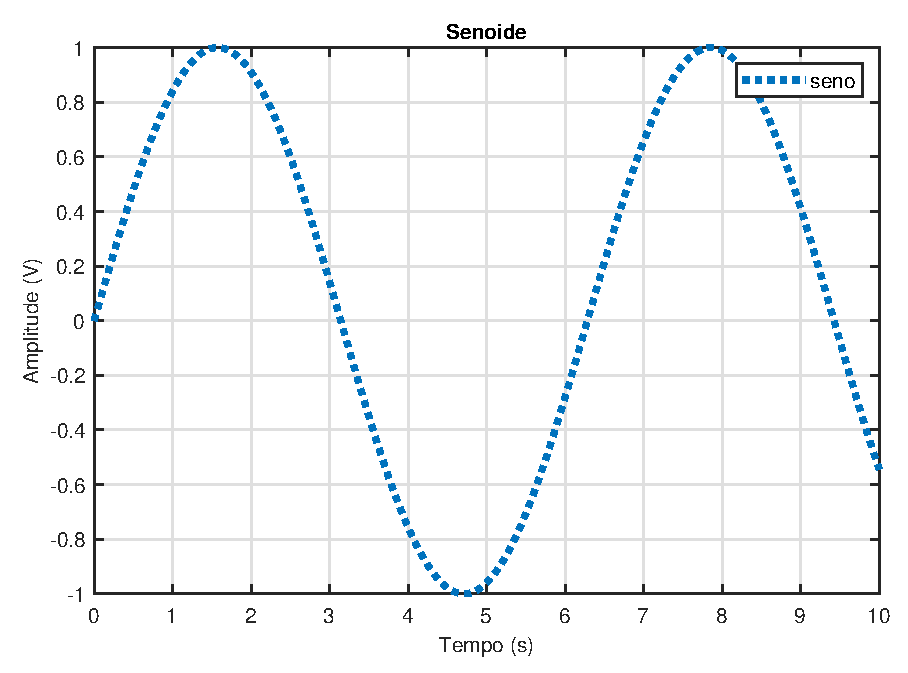
\includegraphics{teste.eps}
    \caption{Caption}
    \label{fig:enter-label}
\end{figure}

Deve Tabela~\ref{tab:jsl07} também elencar algumas equações Equação~\eqref{eq:one} de outros autores que sejam relacionados com a temática do trabalho \cite{INOUE2011}. 
Usm bom esquema para a introdução é \c{c}\~a:



\begin{itemize}
    \item Contextualização do tema (1-2 parágrafos) \cite{JESSICA2011}
    \item Motivação (1-2 parágrafos, mas pode ser junto com o objetivo e diferencial)
    \item Avaliação da literatura (3 a 5 parágrafos)
    \item Objetivo e diferencial do trabalho (1-2 parágrafos)
    \item Organização do trabalho (1 parágrafo) \cite{Joao2011}
\end{itemize}

A organização do trabalho é feita assim: “Na Seção \ref{sec:fundamentacao}, apresenta-se a fundamentação teórica do trabalho. A metodologia desenvolvida é apresentada na Seção \ref{metodologia}

